\newpage
\section{PROCEDIMENTOS METODOLÓGICOS}

Para alcançar o objetivo de classificar os comentários pejorativos em vídeos infantis do Youtube, os passos a seguir descritos na Figura \ref{fig:metodologia} foram planejados. A execução dos passos é descrita no Capítulo 6.


\begin{figure}[H] %use h para forçar que a figura fique abaixo do texto
	\caption{\label{fig:metodologia} Ilustração do procedimento metodológico}
	\begin{center}
	    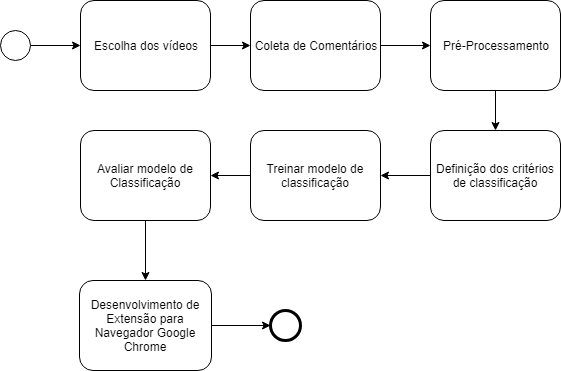
\includegraphics[scale=0.7]{figuras/figura_6.png} % altere o atributo scale para o tamanho da figura
	\end{center}
	\legend{Fonte: autor}
%Verificar se precisa por a data aqui 
\end{figure}


% Mudar o tempo para futuro
\subsection{Escolha dos vídeos}
O principal critério para a escolha do vídeo para este trabalho, é que seu público alvo seja infantil ou adolescente. Naturalmente, quanto mais comentários o vídeo possuir, maior a quantidade de dados para análise, logo o ideal é buscar vídeos infantis que apresentam um número expressivo de comentários, em torno de pelo menos mil. Porém, tendo em consideração que nem sempre é possível encontrar vídeos com essa quantidade ideal de comentários, podem ser utilizados vídeos com menos comentários. A popularidade dos canais que postaram os vídeos é um fator a ser considerado, visto que um canal com maior popularidade, tende a possuir vídeos com mais comentários.


\subsection{Coleta de Dados}
A fim de ter os dados para o ponto de partida da pesquisa e tendo em conta a grande quantidade de comentários em vídeos com público-alvo jovem, foi desenvolvida uma ferramenta em Python para coleta dos comentários em vídeos do Youtube. O objetivo da ferramenta é ser simples e objetiva na coleta desses comentários. A ferramenta é responsável pela etapa de preparação dos dados, dentro dos conceitos de mineração de texto.


\subsection{Pré-Processamento}
Uma vez que os dados armazenados não estão em formato adequado para extração do conhecimento, faz-se necessária a aplicação de métodos para \textit{extração, integração,} \textit{transformação},
% ta mas o que é isso? ai vou precisar olhar no referencial teórico e adaptar conforme o que eu fiz aqui!!!
\textit{limpeza}, \textit{seleção e redução} de volume desses dados, antes da etapa de mineração \cite{morais2007mineraccao}.

Inicialmente, observa-se uma grande quantidade de comentários sem sentido em vídeos infantis no Youtube, compostos quase que inteiramente por espaços em branco ou símbolos e letras aleatórios. Em vídeos destinados à adolescentes, há menor ocorrência de comentários sem sentido. 

Faz necessário a utilização de um método ou ferramenta que fará a limpeza dos textos, bem como a aplicação da ferramenta NLTK para que seja feito o pré-processamento dos textos. Um \textit{script} foi criado pelo autor e sua utilização é detalhada no Capítulo 6.


\subsection{Definição dos Critérios de Classificação}

A classificação dos comentários é definida manualmente, levando em consideração comentários de amostragem, que serão classificados como \textbf{pejorativos} ou \textbf{não pejorativos}. 

Dado a enorme quantidade de comentários coletados, um dicionário de classificação também será criado para a ferramenta \textbf{SentiStrength}, a fim de facilitar a criação do conjunto de treino a ser dado de entrada para gerar o modelo de classificação. 

Após a classificação manual e a classificação assistida utilizando a \textit{SentiStrength}, um modelo deve ser construído a partir do treinamento  com o conjunto de dados coletados, para que se  possa classificar automaticamente os novos comentários obtidos do Youtube.

\subsection{Treinamento do Modelo de Classificação}
O classificador Naïve Bayes recebe um conjunto de dados de treino, e um conjunto de testes para averiguar a precisão do modelo de classificação \cite{ZhangandLi2007Bayes}. Esses conjuntos de dados são escolhidos de forma aleatória dentre os comentários obtidos.

Por meio da ferramenta \textit{Sentistrength}, pode-se obter um grupo de comentários classificados automaticamente, que deve ser analisado e melhorado pelo autor, a fim de obter um modelo de classificação mais preciso.

\subsection{Definição dos critérios de classificação}
A definição dos critérios de classificação corresponde à avaliação do modelo de classificação, ou seja, da sua qualidade.
O modelo gerado poderá ser testado, utilizando os comentários que não foram utilizados na fase de treino, ou seja, utilizando os comentários selecionados para compor o conjunto de teste. 

A avaliação do modelo é feita através da ferramenta \textit{Scikit-learn}, que fornece métodos de \textit{score} prontos para as medidas de \textit{precision} e \textit{recall}.



\subsection{Desenvolvimento de Extensão para Navegador Google Chrome}

Por meio do desenvolvimento de um \textit{plugin} para o Google Chrome é possível utilizar o modelo construído e indicar vídeos com comentários pejorativos.
Nessa etapa, são avaliados os resultados do processamento dos comentários, agregando agora pelos vídeos dos quais foram coletados, indicando quais os vídeos tem maiores taxas de comentários pejorativos e que não são considerados seguros para crianças e adolescentes.

